
\section{Algorithm comparison: searching for periodic signals}
\label{sec:exp_algorithm}

If one were to focus their search on monotransits, no algorithm to determine the period is needed. Any value in the PTS above a certain threshold can be considered as potential detection (see Figure \ref{fig:algorithm-mono_example}). In most attempts of finding new planet candidates, the search is guided by the repetition of transit signals. In the following, we take a closer look at the algorithms described in sections \ref{sec:alg_peaks} and \ref{sec:alg_folding} and refer to these algorithms as PTS-Peak and PTS-Fold respectively \todo{give these name in Methodology already}.

\begin{figure}
    \centering
    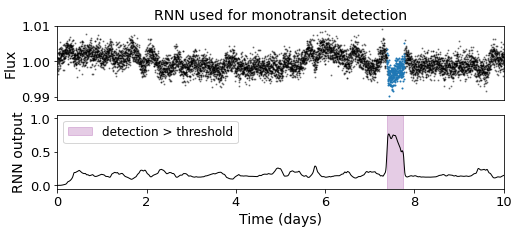
\includegraphics[width=0.6\linewidth]{Experiments/Figures/Algorithm/mono_example.png}
    \caption{\red{[TODO: caption]}}
    \label{fig:algorithm-mono_example}
\end{figure}

Figure \ref{fig:algorithm-both_correct} shows an example LCSim light curve with transit signals from a single planet. Both PTS-Fold and PTS-Peak are able to correctly determine the period $P$ and epoch $t_0$ of the signal, using the PTS produced by the RNN. For PTS-Peak, we have adopted a peak threshold of 0.25. 

In order to search for successes and failure cases of both methods, we had LCSim generate 250 light curves of 27.4 days, each with 3 to 5 transits of a single planet. The first and only run of this experiment resulted in 62 failure cases of both methods. For 12 cases only PTS-Fold was correct, and for 1 case only PTS-Peak was correct because PTS-Fold's predicted $t_0$ was off by 2 hours. One of the cases in which only PTS-Fold was correct is shown in figure \ref{fig:algorithm-peak_fail}. As can be understood from this figure, the peaks in the PTS corresponding to the true signals need to be distinct from the noise for the PTS-Peak to work well. However, sometimes a few transit events could go undetected, false positives might be produced by the RNN, or the peaks are just not strong in general. In those cases, PTS-Peak might match the wrong peaks together, or just prefer smaller periods than the true signal period due to the noise in the PTS.

\begin{figure}
    \centering
    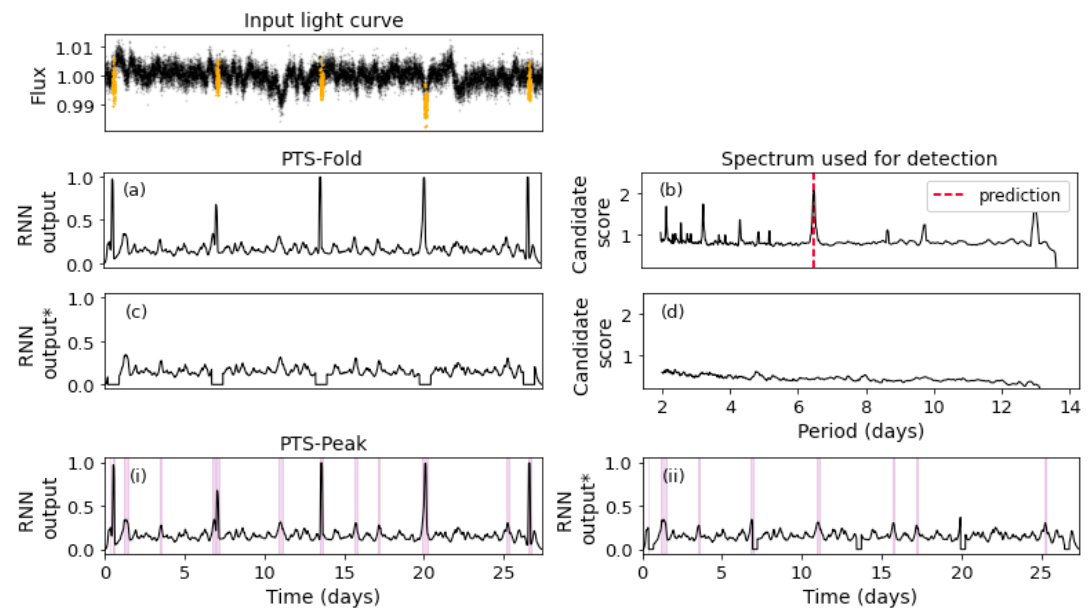
\includegraphics[width=0.9\linewidth]{Experiments/Figures/Algorithm/both_correct.png}
    \caption{\red{[TODO: caption]}}
    \label{fig:algorithm-both_correct}
\end{figure}

\begin{figure}
    \centering
    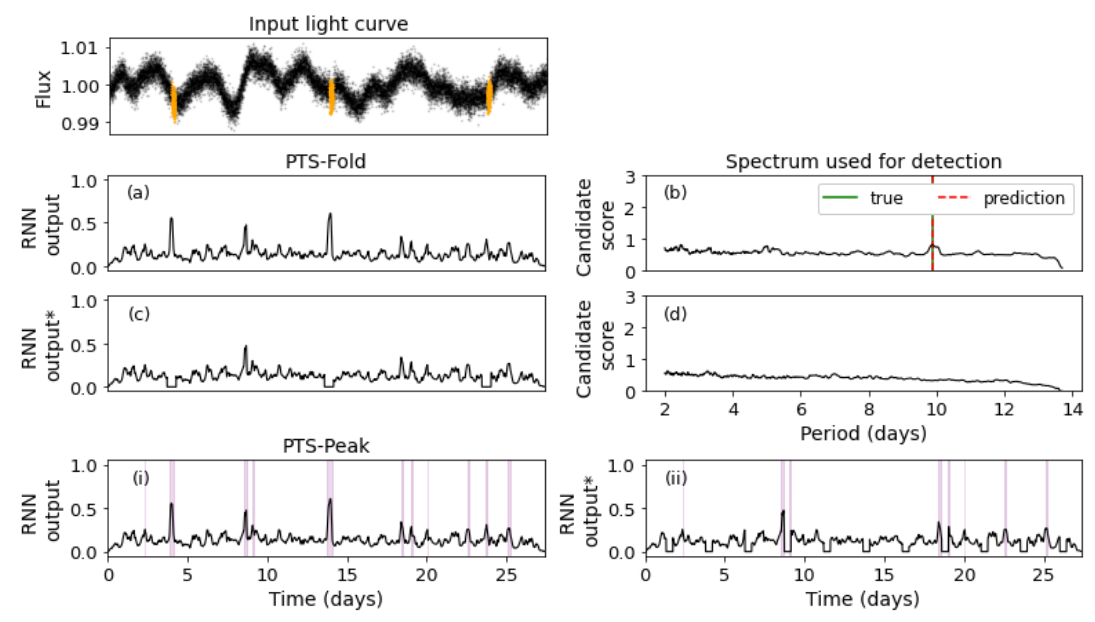
\includegraphics[width=0.9\linewidth]{Experiments/Figures/Algorithm/peak_fail.png}
    \caption{\red{[TODO: caption]}}
    \label{fig:algorithm-peak_fail}
\end{figure}

Nevertheless, in many cases PTS-Peak correctly retrieved the hidden signal. We therefore explore an extension to this method, which has the potential of resolving the issue of mismatching peaks in a given PTS. The network we use for this is the representation network described in Section \ref{sec:extension_repr}. For the sake of illustration, the network was trained to learn 2-dimensional representations of signals. Recall that the network outputs a representation at each time step, so the representation of a signal is the aggregation over several time steps. The angle between two representation vectors represents their dissimilarity, and since the angle does not depend on the magnitudes of the vectors we can visualize the representations of signals on the unit circle.

From best to worse, figures \ref{fig:algorithm-repr1}, \ref{fig:algorithm-repr2} and \ref{fig:algorithm-repr2} illustrate how the use of signal representations could have prevented mismatching of peaks by PTS-Peak that led to incorrect detections. \todo{Describe what else these figures say, e.g. transit depth seems to be captured, can't say much about shapes specifically. further analysis needed in further work}. \todo{explain these results were obtained with simple noisy straight lines with injected transits -- not certain whether these results will hold under disturbing background patterns}.

\begin{figure}
    \centering
    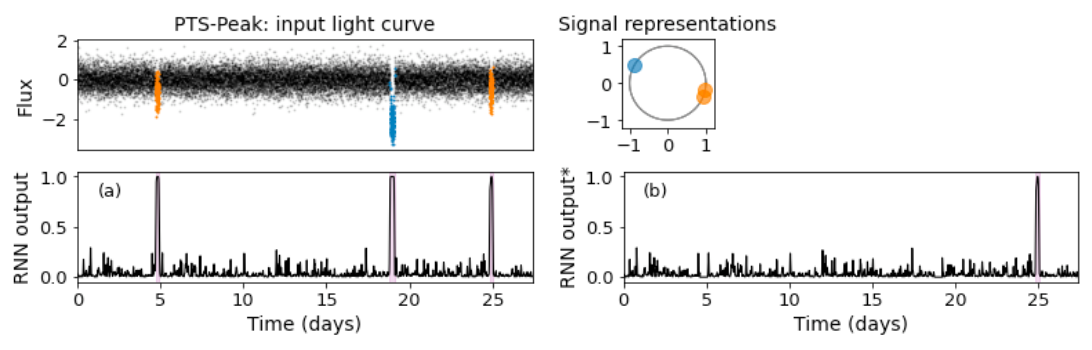
\includegraphics[width=0.9\linewidth]{Experiments/Figures/Algorithm/repr1.png}
    \caption{\red{[TODO: caption]}}
    \label{fig:algorithm-repr1}
\end{figure}

\begin{figure}
    \centering
    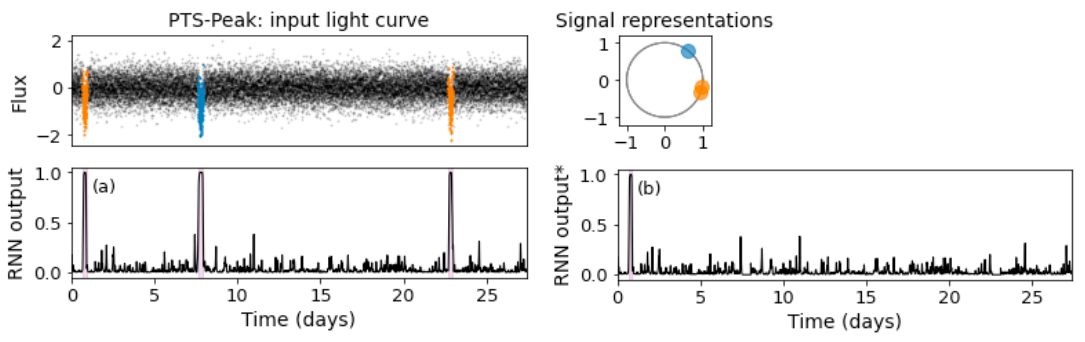
\includegraphics[width=0.9\linewidth]{Experiments/Figures/Algorithm/repr2.png}
    \caption{\red{[TODO: caption]}}
    \label{fig:algorithm-repr2}
\end{figure}

\begin{figure}
    \centering
    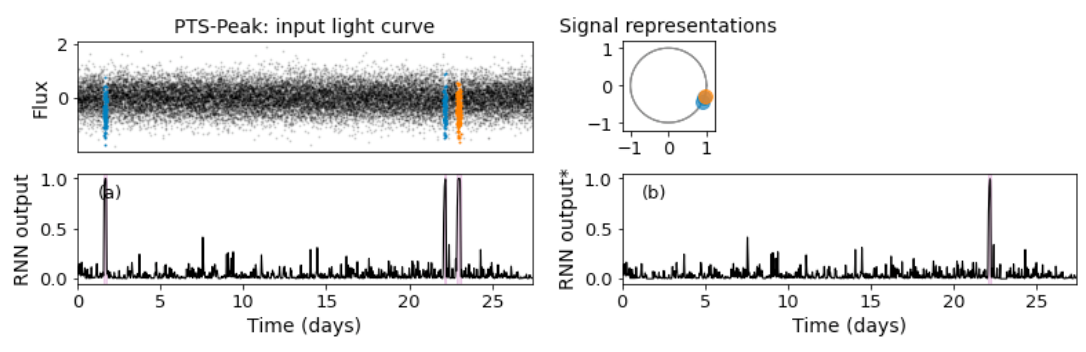
\includegraphics[width=0.9\linewidth]{Experiments/Figures/Algorithm/repr3.png}
    \caption{\red{[TODO: caption]}}
    \label{fig:algorithm-repr3}
\end{figure}
